\documentclass[letterpaper,12pt]{article}
\usepackage[utf8]{inputenc}

\usepackage[T1]{fontenc}
\usepackage{tgtermes} %%%font

\usepackage{geometry}
\usepackage{amsmath}
\usepackage{float}
\usepackage{graphicx}
\usepackage{subcaption}
\usepackage{amssymb}
\usepackage{adjustbox}
\usepackage{wrapfig} %%imagen envuelta por un texto
\usepackage{xcolor}
\usepackage{fancyhdr}
\usepackage{tabularx} %%TABLAS OH YEAH

\title {\textbf{Notas de gestión empresarial}}
\author{Lara Xocuis Martha Denisse}
\date{23 de agosto de 2023}
\geometry{top=2cm, bottom=2cm, left=2cm, right= 2cm} %%margen
\graphicspath{{images/}}
\parindent=0pt

\begin{document}
\maketitle

%%%%%%%%%%%%%%%%%%%%%%%%%%%%%%%%%%%%%%%%%%%%%%%%%%%%%%%%%%%%%%%%%%%%%%%%%%%%
\begin{sloppypar}
\section{Introducción de la materia}
\textbf{Nombre de docente:} Juana Gabriela. 22 91 45 97 57 (contacto)
\vspace{0.3cm}\\
\textbf{Evaluación:}

\begin{table}[H]
    \begin{tabular}{|c|c|} \hline
        Evidencia diaria & 20\% \\ \hline
        Tareas & 40\% \\ \hline
        Proyecto & 40\% \\ \hline
        
    \end{tabular}
\end{table}

Gestionar quiere decir seguir un proceso, enfoque de una administración más amplia.

Podemos tomar la estructura como la siguiente: 
\begin{figure}[H]
    \centering
    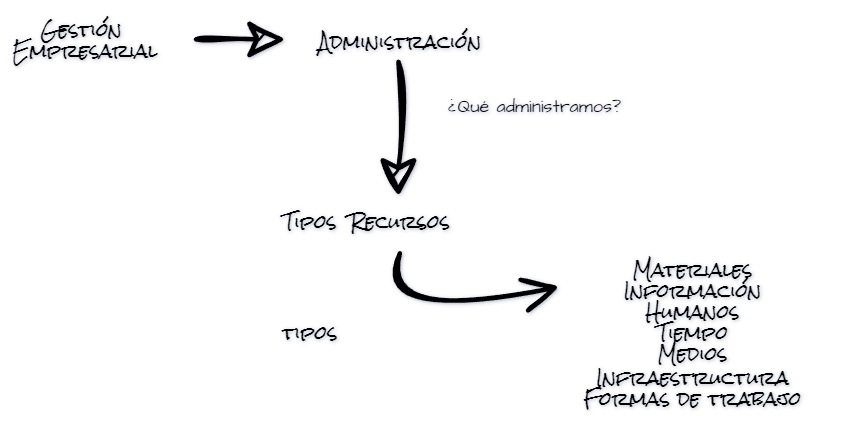
\includegraphics[width=0.8\textwidth]{images/GE.1.png}
\end{figure}
%%%%%%%%%%%%%%%%%%%%%%%%%%%%%%%%%%%%%%%%%%%%%%%%%%%%%%%%%%%%%%%%%%
\newpage 
\subsection*{Lara Xocuis Martha Denisse.}
Clase de 24 de agosto de 2023.
\textbf{\textcolor[rgb]{0.5,0.5,0.3}{\section{¿Es el beneficio la medida de la eficiencia?}}} %%color

El \textbf{beneficio }es una relación entre el ingreso, ventas, costo de producto, mermas, desperdicios, ingresos, número de empleados, demanda de productos e inventario. Podemos decir que si, el beneficio es la medida de la eficiencia.
\vspace{0.3cm}\\
\textbf{Palabras clave de estrategia : plan, fin, proceso, tiempo determinado, recursos, objetivo/meta. }

\subsection*{Definición propia de estrategia dentro del ambito empresarial/administración. }
Una estrategia es un proceso el cual se toman en cuenta de forma minuciosa los recursos y tiempo para alcanzar una meta determinada. Esto nos ayuda a ver de una forma más objetiva, amplia y optimizada todo lo que está a nuestro alcance para poder llevar a cabo el plan a realizar dicha meta. 

\subsection*{Definición más acertada de estrategia. (investigación)}
\begin{itemize}
    \item Una estrategia se define como actividades de planeamiento a largo plazo, guiadas por valores definidos y constantes en el
    tiempo. Este mismo contribuye a actividades ordenadas y con un propósito.
\end{itemize}
\textit{-Fundamentos de gestión empresarial pag. 42 [LIBRO]}
\vspace{0.3cm}\\
Entre los diferentes autores que definen la "estrategia", a continuación los que más me parecieron interesantes:
   \begin{itemize}
    \item Alfred Chandler (historiador de la economía estadounidense,1962, p.13) que la define como "la determinación de los objetivos básicos a largo plazo y los fines de una empresa, la adopción de cursos de acción y la asignación de recursos necesarios para alcanzar estos objetivos"
    \item Una muy conocida y celebrada es por Kenneth R. Andrews, para el "la estrategia es el patrón de los principales objetivos, propósitos o metas, políticas y planes esenciales para conseguir dichas metas, establecidos de tal manera que definan en qué clase de negocio la empresa está o quiere estar y qué clase de empresa es o quiere ser"  (escribió el pensamiento sobre la política de negocio o estrategia corporativa en la Escuela de Negocios de Harvard, 1977, p-59)
   \end{itemize}
\textit{ - En torno al concepto de estrategia. Díez de Castro, Emilio Pablo Martín Jiménez, Francisca de Asis . Universidad de Sevilla. Departamento de Administración de Empresas y Comercialización e Investigación de Mercados (Marketing)
Artículos (Administración de Empresas y Comercialización e Investigación de Mercados(Marketing). 1992) [ARTÍCULO]}

\subsection*{Definición propia de cliente}
El cliente es la potencia de la empresa, su forma de visión, manejo y adaptación de estrategias que se deben replantear con el fin de satisfacer las necesidades de dicho cliente.

%%%%%%%%%%%%%%%%%%%%%%%%%%%%%%%%%%%%%%%%%%%%%%%%%%%%%%%%%%%%
\newpage
\subsection*{Lara Xocuis Martha Denisse.}
Clase de 25 de agosto de 2023.
\textcolor[rgb]{0.5,0.5,0.3}{\section{El cliente}}
Punto medular de la riqueza de la empresa. 

UV Clase (E.E) $\longrightarrow$ entrada de alumnos y maestr@, se necesita:
\begin{itemize}
    \item Aprobar
    \item Aprender
    \item Madurez
\end{itemize}
Para lograr estos objetivos es importante tener en cuenta que el maestr@ y alumno necesitan para el proceso:
\begin{itemize}
    \item Estudiar
    \item Enseñanza 
    \item Asistencia 
    \item Atención
    \item Participación 
    \item Compromiso mutuo 
    \item Tarea. Evidencia 
\end{itemize}
Alumnos (\textbf{Clientes con requisitos}), ¿qué quieren?
\begin{itemize}
    \item Más comunicación, participación 
    \item Más dinámica entre clases
    \item Integración del grupo, integración mutua
    \item Clases amenas, no aburridas 
    \item Material
    \item Tareas, proyectos necesarios 
    \item Convivencia respetuosa
    \item Compromiso
    \item Disciplina 
\end{itemize}
\textcolor[rgb]{0.5,0.5,0.3}{\section{VALOR.}}
\begin{itemize}
    \item ¿Qué es el valor?. El valor creado para el cliente es la diferencia entre el valor que éste asigna al producto o servicio  -el máximo que estaría dispuesto a pagar - y el precio que realmente abona por él. Se le puede decir también como la importancia que se le concede a una cosa o acción determinada. 
    \vspace{0.3cm}\\
    - ¿Qué es crear valor para el accionista?: 
    \item ¿Cuál es el valor de esta clase? Pararse temprano y optar con una actitud de responsabilidad, tener puntualidad y dedicarle el tiempo necesario a la clase, es decir, estar dispuesto a tener ciertos sacrificios para un mejor alcance. 
\end{itemize}\newpage
\section*{Tarea 1. Lara Xocuis Martha Denisse. 26/08/23}
\textbf{1. Diferencias existentes entre una organización que busca beneficios y otra que no.}
\begin{table}[H]
    \centering
    \begin{tabular}{|m{0.42\linewidth}|m{0.42\linewidth}|} 
        \hline
        organización que busca beneficios & organización que no busca beneficios\\
        \hline
        \begin{itemize}
            \item Buscan innovar, mejorar y crecer
            \item Tener mejores servicios 
            \item Aumentar ingresos 
            \item Impulsar la gestión de la empresa 
            \item Se valen de recursos materialistas
        \end{itemize}
        & 
        \begin{itemize}
            \item Objetivo del tipo social y altruista 
            \item Suele ser voluntario 
            \item No buscan recaudar ingresos para un beneficio propio (como accionistas)
        \end{itemize} \\ 
        \hline 
    \end{tabular}
\end{table}
\textbf{2. Cite algunos ejemplos de ambas y describa brevemente las diferencias más importantes.}
\begin{itemize}
    \item Coca cola (en busca de beneficios): Ingresos dominantes en base a sus productos, producen y comercializan de forma global, emplean una jerarquía dentro de las distribuciones de trabajo en la empresa, reparten las ganancias entre sus empleados y con eso potencializan la empresa para buscar más objetivos con el fin de imponerse contra la competencia.
    \item Greenpeace (no busca beneficios): reciben donaciones o acciones caritativas para ayudar contra el calentamiento global, consumismo y el cuidado ecológico, tienen una administración y desempeño transparente, es humanitario/activista y busca fortalecer la integración de las comunidades, no obtienen ganancias materialistas para su propio beneficio
\end{itemize}
\textbf{3. Realice además un breve comentario sobre como puede una organización no orientada a beneficios distribuir recursos a la sociedad en general.} 
\vspace{0.3cm}\\
Comúnmente buscan recaudar donaciones o aportaciones que las personas les dan de manera individiual con el fin de invertirlo para solucionar ciertos problemas sociales sin tener un compromiso económico o político, estas donaciones no solo pueden ser dinero, también suele ser el tiempo en que aportan las personas de forma voluntaria en donde comunmente se realizan movimientos activistas. 
\vspace{0.3cm}\\
\textbf{4. ¿Podría describir usted algún ejemplo de alguna empresa que haya alcanzado un producto nuevo al mercado y la repercusión que este ha tenido en la calidad de vida de las personas?}
\vspace{0.3cm}\\
En cuestión de tecnologia podemos hablar de las primeras computadoras lanzadas al mercado por UNIVAC (NIVersAl Computer) en 1951, aunque ya se había creado el primer ordenador desde antes, esta compañía  y en conjunto de General Electric fue la primera en comercializarlas. Su impacto tecnológico fue tan grande que hoy en día existen distintas empresas en función de competencia para crear portatiles y diversos dispositivos inteligentes que cada día son más optimizados. Afortunadamente este producto tuvo mucho éxito por lo que en la actualidad podemos decir que una computadora es casi indispensable para nuestro día a día.
\newpage
\textbf{Es importante reflexionar sobre los problemas de INTRODUCIR nuevos productos en el mercado.Imagínese que usted es el director de marketing de una empresa que desea lanzar al mercado una nueva forma de producir energía eléctrica, por ejemplo un generador de energía solar para granjas y fábricas.}
\vspace{0.3cm}\\
\textbf{¿Cuáles serían las ventajas para los usuarios?}
\begin{itemize}
    \item La optimización de producción respecto a los proveedores de energía, productos más "organicos" respecto a su creación (en cuestión de fábricas.)
\end{itemize}
\textbf{¿Qué problemas existirían para mantener las instalaciones?}
\begin{itemize}
    \item Tomando en cuenta en cuantos se necesitan para empezar a comercializar, se pueden tener problemas de producción en cuestión de materiales y precios, si se enfocan en reducir costos de proovedores de materiales solo para no hacer inversiones tan grandes -como ejemplo- la calidad de los generadores baja y eso puede venir junto a un mal funcionamiento en los productos, y por tanto, bajan las ventas. Es por eso que la mayoría de productos son muy elevados de precio, sin embargo, si resulta muy beneficioso para los clientes obtener dichos productos, entonces habrá una empresa estable.  
\end{itemize}
\textbf{¿Qué métodos emplearía para eliminar o reducir los problemas de lanzamiento? }
\begin{itemize}
    \item Contar con buena publicidad y marketing, buenos accionistas, materiales y premisas favorables para los clientes.
\end{itemize}
\section*{Preguntas}
\textbf{1. ¿Con qué recursos cuenta una empresa para obtener beneficios?} Accionistas, capital de base para invertir y potencializar otras cosas, manufactura, empleados, maquinaria, infraestructura. 
\vspace{0.3cm}\\
\textbf{2. ¿Cuál es la diferencia entre una organización privada y otra del sector público?} La del sector público comúnmente es parte del gobierno, invierten con el fin de dar mejores instalaciones y dar servicios a la comunidad.  Por otra parte las de sector privado se basan en su propia estrategia para sus propios beneficios con el fin mantener su sostenibilidad y competencia en el mercado 
\vspace{0.3cm}\\
\textbf{3. ¿Qué motivaciones crean los beneficios en un empresario?}A seguir invirtiendo e innovando cosas, se mantienen en una actitud enfocada al crecimiento de su empresa. 
\vspace{0.3cm}\\
\textbf{4. ¿De qué forma contribuyen los beneficios de una empresa en el bienestar de la sociedad? } En ofrecer mejores empleos y productos en cuestión de salario y calidad. También parte de las ganancias de la empresa pueden aportar mejores servicios e infraestructuras para nuevos productos, gracias a esto suelen originarse muchas formas de estrategias de marketing y distribución.
\vspace{0.3cm}\\ 
\textbf{5. ¿Cómo crea sus clientes una empresa?} Una empresa se moldea en base a los beneficios que espera conseguir el cliente, esta debe identificar las necesidades y las formas de tratarlos como es debido, debe tratar por todos los medios en que un cliente se sienta satisfecho, 
\vspace{0.3cm}\\ 
\textbf{6. ¿De qué forma afrontará la empresa los cambios que se están produciendo?} Gracias al marketing y la innovación se puede investigar de forma minuciosa el mercado mediante un análisis sobre el perfil de los clientes, cosas sobre tendencias de consumo, su competencia, publicidad, diseño o acciones de producción deben ser su foco para las oportunidades que desean en el futuro. 
\vspace{0.3cm}\\ 
\textbf{7. ¿Cómo afectan los cambios económicos en la gestión de una empresa? } En la gestión de productos, servicios y financiación de compras por clientes.
\vspace{0.3cm}\\ 
\textbf{8. ¿Cuáles son las responsabilidades de un empresario en materia de Marketing? } Análisis sobre perfiles de los clientes, actitudes sociales, conductas psicológicas y tendencias de compras. También sobre el diseño de políticas de precios y productos, envansado, comercialización y logística.
\vspace{0.3cm}\\ 
\textbf{9. ¿Cuál es la diferencia entre invención e innovación? }
\begin{itemize}
    \item \textbf{invención:} diseño y desarrollo de nuevas tecnologías, y por ende, nuevos productos. 
    \item \textbf{innovación:} evolución económica de la empresa sobre las oportunidades en las que basa su futuro.
\end{itemize}

\newpage
\subsection*{Lara Xocuis Martha Denisse.}
Clase de 30 de agosto de 2023.

\textcolor[rgb]{0.5,0.5,0.3}{\section*{Definición de Administración}}
La definición es un \textbf{proceso : }
\begin{itemize}
    \item Planear 
    \item Organizar 
    \item Dirigir
    \item Controlar 
\end{itemize}

\textbf{¿Qué es un organigrama?} Dibujo de líneas de dirección de la empresa. $\longrightarrow$ ¿Dónde está el administrador? $\longrightarrow$ ¿Por qué está ahí?
\vspace{0.3cm}\\ 
Habilidades y competencias de un Administrador 
\begin{itemize}
    \item Perfil del puesto 
    \item Instrumento de evaluación a candidatos (puede haber más de uno)
\end{itemize}

\section*{FAURECIA}
\begin{enumerate}
    \item Investigar faurecia
    \item Habilidades y competencias de un administrador
    \item Diseñar perfil de puesto, investigar que es, formato, creación
    \item Como evaluar los candidatos   
\end{enumerate}

\section*{ENTREGABLES}. 1 archivo PDF 
\begin{itemize}
    \item Portada $\longrightarrow$ índice 
    \item Introducción
    \item Hablar de faurecia
    \item Competencias y habilidades del adminsitrador de Faurecia. ¿Por qué? 
    \item Diseño del perfil. Explicación
    \item Formato (Dibujo) - ¿Qué esperamos de este formato? 
    \item Instrumentos de evaluación a candidatos (entrevistas, exámenes psicométricos, etc) se tienen que justificar este tipo de instrumentos
    \item Conclusiones individuales
    \item Aprendizaje individual de la actividad
    \item Bibliografía 
    \item Anexos
\end{itemize}
\newpage
\subsection*{Lara Xocuis Martha Denisse.}
Clase de 8 de septiembre de 2023.
\section{Ingeniería}
\begin{figure}[H]
    \centering
    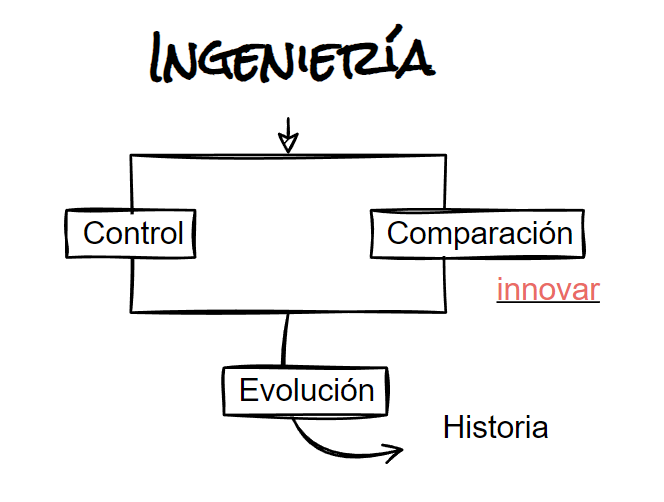
\includegraphics[width=0.4\textwidth]{images/ola .png}
\end{figure}


\begin{enumerate}
    \item Escuela clásica (el momento ) / tradicional 
    
    \item Escuela empírica
    
    \item Escuela comportamental 
    
    \item Escuela teoría de decisión 
    
    \item Escuela gestión de sistemas
    \item Gestión del conocimiento 
    \item Maquila 
    \item Justo a tiempo 
    \item Clústers industriales 
    \item Globalización 
    \item Alianzas estratégicas 
    \item Organizaciones virtuales 
    \item Franquicias
    \item e-commerce 
    \item teoría de restricciones 
    \item admón del tiempo 
    \item pensamiento sistémico 
    \item coaching 
    \item misión, visión, valores 
    \item titularización 
    \item gerencia / evaluación de proyectos / gestión ambiental 
\end{enumerate}

\newpage
\subsection*{Lara Xocuis Martha Denisse.}
Clase de 20 de septiembre de 2023
\vspace{0.3cm}\\ 
Historia de las tecnologías en la administración

El concepto de administración tecnológica

Importancia de la administración tecnológica

Funcionalidad de la administración tecnológica

Planes, estrategias y políticas tecnológicas

\newpage
\subsection*{Lara Xocuis Martha Denisse}
Clase 21 de septiembre de 2023

\begin{itemize}
    \item ¿Qué es una PyME? 
    \item // MiPyMe 
    \item Indicadores
    \item Organización del lugar c: 
\end{itemize}

Tareas de un administrador
\begin{itemize}
    \item Planear 
    \item Organizar 
    \item Dirigir 
    \item Controlar
\end{itemize}
\newpage
\subsection*{Lara Xocuis Martha Denisse}
Clase 18 de octubre de 2023
\textcolor[rgb]{0.5,0.5,0.3}{\section*{El cliente}}

¿Quién es el cliente?
Los clientes constituyen el eje principal de cualquier empresa. El punto de partida de las técnicas de \textbf{marketing} y del \textbf{plan de acción empresarial} es el análisis de las características del cliente y la determinación de perfiles que permitan clasificar a los clientes en grupos, adoptar medidas de atención específicas y posibilitar \textbf{el establecimiento de pautas de actuación} adecuadas para la consecución de un servicio de calidad.
\vspace{0.3cm}\\
Este mismo estudio debe ser periódico para adaptar adecuadamente las pautas y cambios surgidos en las necesidades de los clientes.
\vspace{0.3cm}\\
Los continuos cambios en el entorno, en el diseño de productos, etc., determinan los cambios en los gustos, necesidades, motivaciones y expectativas de los clientes.
\vspace{0.3cm}\\
Es importante saber la diferencia entre \textbf{consumidor, cliente y usuario}: 
\begin{center}
    Consumidor: Persona que compra un producto o servicio.\\
    Cliente: Persona que compra habitualmente en la misma empresa\\
    Usuario: Persona que disfruta habitualmente de un servicio o del empleo de un producto.
\end{center}
\begin{itemize}
    \item Demografía: La segmentación demográfica es dividir el mercado en grupos de consumidores con base a variables demográficas. Utilizando variables como edad, sexo, tamaño y ciclo de vida de la familia, nivel de ingresos, raza, ocupación, nivel educativo y nacionalidad.
    En efecto, las variables demográficas son datos de población importantes que pueden ser usados para crear perfiles de consumidores. Estas variables se utilizan mucho en la segmentación de mercado porque resultan muy fáciles de medirse. Además, se relacionan con la demanda que es un aspecto muy importante para cualquier empresa.

    Por lo tanto, las variables demográficas son las que se usan más comúnmente en el proceso de segmentación de mercado. Dado que son las variables más fáciles de identificar y de medir.
    
    Variables más usadas:
    \begin{itemize}
        \item Edad 
        \item Sexo 
        \item Tamaño de la familia
        \item Ciclo de vida de la familia 
        \item Nivel de ingresos
        \item Ocupación 
        \item Nivel educativo
        \item Religión, raza y nacionalidad
    \end{itemize}

    \item Geografía: Hace referencia a la división del marcado tomando en cuenta las diferencias geográficas entre un lugar y otro, a la hora de distribuir los productos o servicios. La segmentación geográfica ayuda a recopilar y analizar información de acuerdo a la ubicación física de las personas.
    
    Esta clase de segmentación es una importante fuente de datos para la comercialización, para saber los lugares indicados para vender o realizar campañas de publicidad. La segmentación geográfica divide a los mercados en diferentes unidades geográficas y esto es importante porque las características de los consumidores son diferentes.

    Las empresas consideran importante la segmentación geográfica cuando la ubicación de los clientes es diferente, para ello, debe considerar las diferencias culturales que existen entre una zona y otra a la hora de envasar, transportar y distribuir el producto.

    \item Psicografía: toma en cuenta los rasgos psicológicos de los consumidores, su estilo de vida, sentimientos, intereses, deseos, etc. Cada vez está siendo más utilizada por negocios que quieren alcanzar realmente a su consumidor ideal y dar en el blanco.

    Es una forma de seccionar a tu grupo de consumidores actuales y potenciales considerando detalles de su personalidad, su estilo de vida, sus deseos y anhelos, sus sentimientos e intereses, así como sus motivaciones.

    Mientras más informaciones tengamos sobre los aspectos que nos sean útiles, mejor será.

    La segmentación psicográfica es extremadamente necesaria para que una marca pueda crear una relación sólida con su consumidor.

    Al conocer mejor nuestro grupo de consumidores es posible crear una estrategia de comunicación más efectiva y que lo pueda alcanzar más fácilmente.
    \vspace{0.3cm}\\
    ¿Qué analiza?
    \begin{itemize}
        \item personalidad;
        \item valores;
        \item actividades;
        \item pasatiempos;
        \item prioridades;
        \item estilo de vida;
        \item rasgos psicológicos;
        \item creencias;
        \item motivaciones;
    \end{itemize}
    \item Tecnología: adica en su capacidad para proporcionar a los compradores una forma más eficaz de interactuar con sus marcas preferidas. Asimismo, también permite a las empresas racionalizar el proceso de interacción con sus clientes, optimizando así la gestión empresarial.
    
    Para los gerentes de negocios, esta herramienta es especialmente valiosa, ya que agrega un valor significativo al dado que ayuda a las empresas a comunicarse de manera más efectiva con sus clientes. Proporcionando una experiencia de atención al cliente mucho más fácil y satisfactoria para ambas partes.
    \vspace{0.3cm}\\ 
    ¿Como aumenta la productividad empresarial?
    \begin{itemize}
        \item Agiliza los procesos
        \item Mejora la comunicación
        \item Ayuda a los empleados a ser más eficientes
    \end{itemize}
    \item Comportamiento: es el análisis de los diferentes factores que influyen en la conducta de una persona o grupo de personas, al momento de realizar la compra de un producto o servicio. En un sentido un poco más amplio, se trata de entender cómo una persona decide utilizar sus recursos disponibles (tiempo, dinero y esfuerzo) para satisfacer sus necesidades.
    No se trata sólo de saber cómo es el comportamiento del consumidor con respecto a la decisión de compra, sino sobre todo lo que incluye cada una de las etapas del proceso de compra.

    \item Necesidades:  consiste en aquello que motiva a un cliente a comprar un producto o servicio. La necesidad puede ser conocida (es decir, el cliente puede expresarla con palabras) o desconocida, y es el factor que determina qué solución compra el cliente.
    
    No es tan difícil comprender las necesidades del cliente; se trata de factores que influyen en su proceso de decisión de compra en torno a un determinado producto o servicio.

    Las necesidades del consumidor según Maslow son aquellas que resultan comunes a todas las personas al momento de adquirir un producto o servicio, y consisten en necesidades fisiológicas, de seguridad, pertenencia, estima y la autorrealización, así como la espiritualidad.
    \vspace{0.3cm}\\ 
    Tipos de necesidades del cliente 
    \begin{itemize}
        \item Funcionales: son las más tangibles y obvias de los tres tipos principales de necesidades de los clientes. Los clientes suelen evaluar las posibles soluciones basándose en si les ayudarán a realizar una tarea o función concreta. El producto o servicio que mejor responda a su necesidad funcional será probablemente el que compren o contraten.
        \item Sociales:  es una necesidad del cliente relacionada con la forma en que una persona quiere ser percibida por los demás cuando utiliza un producto o servicio. 
        \item Emocionales:se refieren a cómo quiere sentirse el cliente.

        Aunque las necesidades emocionales pueden ser difíciles de precisar, las empresas que identifican las de sus clientes pueden utilizar la información para adaptar y optimizar el mensaje de sus productos.
    \end{itemize}

\end{itemize}
\newpage
\subsection*{Lara Xocuis Martha Denisse}
Clase 19 de octubre de 2023

Describe a tu cliente más valioso.


\end{sloppypar}
\end{document}